\providecommand{\main}{..}
\documentclass[../cmpe-251-project-report.tex]{subfiles}
\externaldocument{1-introduction}
\externaldocument{2-dataset-properties}
\externaldocument{4-clustering}
\externaldocument{5-predictors}
\externaldocument{6-actionable-conclusions}

\begin{document}
  \chapter{Attribute Selection and Ranking}
  \label{ch:selection-ranking}
  To improve clustering results and prediction accuracy, a tree ensemble leaner was used to filter out unimportant attributes. The math formula node and sorter node helped determine which attributes could be removed based on their importance in level 0 of the decision trees in model. The procedure used involved running the workflow (\cref{fig:selection-ranking-workflow}), removing attributes with 0 importance (level 0), and repeating the steps until all attributes had non-zero importance.
  \begin{figure}
    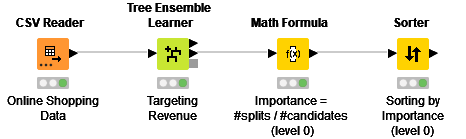
\includegraphics{img/selection-ranking-workflow.png}
    \caption{KNIME workflow used for attribute selection and ranking.}
    \label{fig:selection-ranking-workflow}
  \end{figure}
  The results of the attribute selection and ranking can be summarized in \cref{tab:attribute-selection} and \cref{tab:attribute-ranking} respectively.
  \begin{table}
    \caption{Selection of attributes based on importance (level 0).}
    \label{tab:attribute-selection}
    \begin{tabular}{ll}
      \toprule
      Important Attributes     & Unimportant Attributes \\
      \midrule
      Administrative           & Browser                \\
      Administrative Duration  & Informational          \\
      Bounce Rates             & Informational Duration \\
      Exit Rates               & Month                  \\
      Page Values              & Operating Systems      \\
      Product Related          & Region                 \\
      Product Related Duration & Special Day            \\
                               & Traffic Type           \\
                               & Visitor Type           \\
                               & Weekend                \\
      \bottomrule
    \end{tabular}
  \end{table}
  The important attributes from \cref{tab:attribute-selection} will be the only ones used during cluster analysis and prediction model building to be described in the following chapters.

  Qualitatively, "Informational" type pages don't really help with sales. Neither do the attributes relating to the time of visiting nor ``how'' someone is visiting the site. It seems like the main reasons leading to a purchase lies in the content of certain pages and the metrics for measuring a visitor's journey through Nozama's website.
  \begin{table}
    \caption{Ranking of attributes based on importance (level 0).}
    \label{tab:attribute-ranking}
    \begin{tabular}{lrr}
      \toprule
      Attributes               & Importance (level 0) & Rank \\
      \midrule
      Page Values              & 1.00                 & 1    \\
      Exit Rates               & 0.85                 & 2    \\
      Product Related Duration & 0.61                 & 3    \\
      Product Related          & 0.47                 & 4    \\
      Bounce Rates             & 0.30                 & 5    \\
      Administrative           & 0.24                 & 6    \\
      Administrative Duration  & 0.11                 & 7    \\
      \bottomrule
    \end{tabular}
  \end{table}
  From \cref{tab:attribute-ranking}, the two most important attributes seem to be ``Page Values'' and ``Exit Rates'', which agrees with the observations from~\cref{ch:dataset-properties}.
\end{document}
